% !TeX program = pdfLaTeX
\documentclass[12pt]{article}
\usepackage{amsmath}
\usepackage{graphicx,psfrag,epsf}
\usepackage{enumerate}
\usepackage{natbib}
\usepackage{textcomp}
\usepackage[hyphens]{url} % not crucial - just used below for the URL
\usepackage{hyperref}
\providecommand{\tightlist}{%
  \setlength{\itemsep}{0pt}\setlength{\parskip}{0pt}}

%\pdfminorversion=4
% NOTE: To produce blinded version, replace "0" with "1" below.
\newcommand{\blind}{0}

% DON'T change margins - should be 1 inch all around.
\addtolength{\oddsidemargin}{-.5in}%
\addtolength{\evensidemargin}{-.5in}%
\addtolength{\textwidth}{1in}%
\addtolength{\textheight}{1.3in}%
\addtolength{\topmargin}{-.8in}%

%% load any required packages here



% Pandoc citation processing


\begin{document}


\def\spacingset#1{\renewcommand{\baselinestretch}%
{#1}\small\normalsize} \spacingset{1}


%%%%%%%%%%%%%%%%%%%%%%%%%%%%%%%%%%%%%%%%%%%%%%%%%%%%%%%%%%%%%%%%%%%%%%%%%%%%%%

\if0\blind
{
  \title{\bf Climbing}

  \author{
        Author 1 \\
    \\
     and \\     Author 2 \\
    \\
     and \\     Author 3 \\
    \\
      }
  \maketitle
} \fi

\if1\blind
{
  \bigskip
  \bigskip
  \bigskip
  \begin{center}
    {\LARGE\bf Climbing}
  \end{center}
  \medskip
} \fi

\bigskip
\begin{abstract}
This manuscript\ldots{} The main results are\ldots{}
\end{abstract}

\noindent%
{\it Keywords:} sport climbing, scoring system
\vfill

\newpage
\spacingset{1.45} % DON'T change the spacing!

\hypertarget{introduction}{%
\section{Introduction}\label{introduction}}

(Copy from Rnw + Edit)

\hypertarget{sport-climbing}{%
\subsection{Sport Climbing}\label{sport-climbing}}

\hypertarget{other-scoring-systems}{%
\subsection{Other Scoring Systems}\label{other-scoring-systems}}

\hypertarget{data-and-methods}{%
\section{Data and Methods}\label{data-and-methods}}

We collected data on major climbing competitions from 2018 to 2020,
including the 2020 Continental Championships of Europe, Africa, Oceania,
Pan-America; 2019 and 2018 World Championships; 2018 Asian Games; and
2018 Asian Games.

\hypertarget{results}{%
\section{Results}\label{results}}

\hypertarget{simulations-uniform-ranks}{%
\subsection{Simulations: Uniform
Ranks}\label{simulations-uniform-ranks}}

We conducted a simulation study to examine the rankings and scoring for
climbers in both qualification and final rounds. For each round, we
performed 10000 simulations, and this was accomplished by randomly
assigning the ranks of each event to every participant, with the
assumption that the ranks are uniformly distributed. After the
completion of the simulations, we calculated the final scores for every
simulated round, as well as the final standings for the climbing
athletes. This data would then enable us to answer questions about
various topics, including the distributions of scores for qualifying and
final rounds, and the probabilities of advancing to the finals or
winning a medal, given certain conditions.

\begin{figure}
\centering
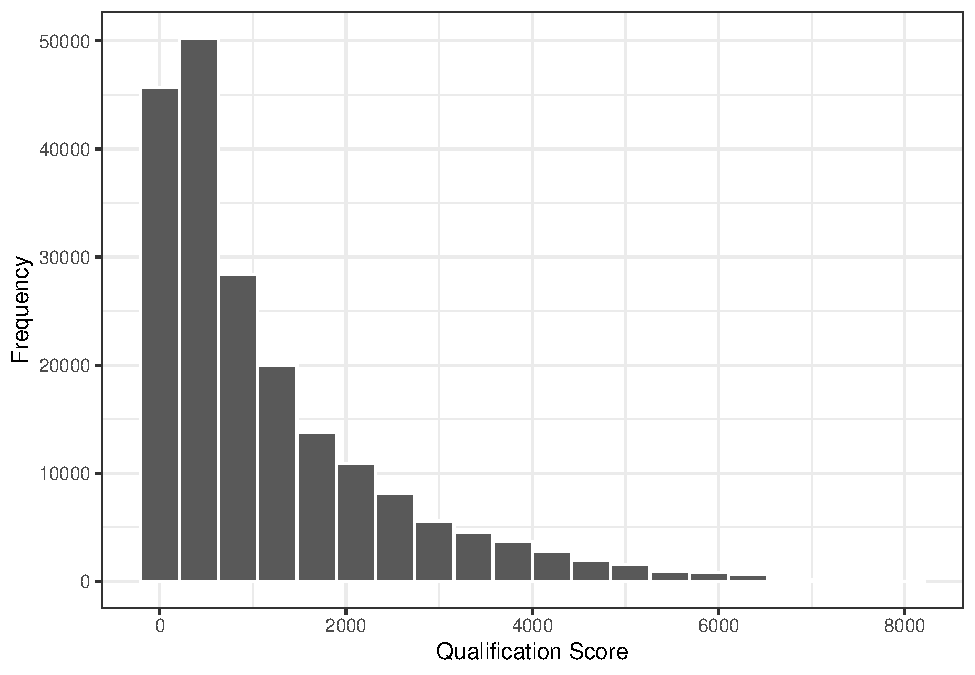
\includegraphics{draft_files/figure-latex/unnamed-chunk-4-1.pdf}
\caption{Distribution of qualification scores}
\end{figure}

For the qualification round, a climber is almost guaranteed to make the
final round if they win the first event (with a 99.51\% chance of
advancing) or if they win at least one of the three climbing
concentrations (99.48\%). On the other hand, finishing last in the first
event or in any event would certainly hurt an athlete's chance of
finishing in the top 8, as the probabilities of a climber advancing
given they finish last in the first and in any event are 0.1830 and
0.1885, respectively. In addition, the average score for qualification
positions 1 to 8 are displayed in Table 1. We notice that on average,
the minimum score that one should aim for in order to move on to the
final round is 435 (for 8th rank).

\begin{table}[ht]
\centering
\caption{Average score for each qualifying rank} 
\begin{tabular}{rr}
  \hline
qual\_rank & avg\_adv\_score \\ 
  \hline
  1 & 36.02 \\ 
    2 & 73.61 \\ 
    3 & 115.40 \\ 
    4 & 162.23 \\ 
    5 & 216.00 \\ 
    6 & 278.16 \\ 
    7 & 350.33 \\ 
    8 & 434.59 \\ 
   \hline
\end{tabular}
\end{table}

Regarding the finals, a climber is very likely to earn a medal (finish
in the top 3) if they win the first event (83.03\% chance) or any event
(85.01\%). In order to obtain a climbing medal, the average score for
getting gold, silver, and bronze are 9.6748, 20.4143, and 33.2648,
respectively (Table 2). A notable trend we observe for both
qualification and final rounds is as the rank increases, the
distribution of the scores becomes more spread out. (Figure\ldots,
facet)

\begin{table}[ht]
\centering
\caption{Average score of medalists} 
\begin{tabular}{rr}
  \hline
final\_rank & avg\_score \\ 
  \hline
  1 & 9.67 \\ 
    2 & 20.41 \\ 
    3 & 33.26 \\ 
    4 & 50.59 \\ 
    5 & 74.76 \\ 
    6 & 110.05 \\ 
    7 & 164.43 \\ 
    8 & 265.78 \\ 
   \hline
\end{tabular}
\end{table}

\begin{figure}
\centering
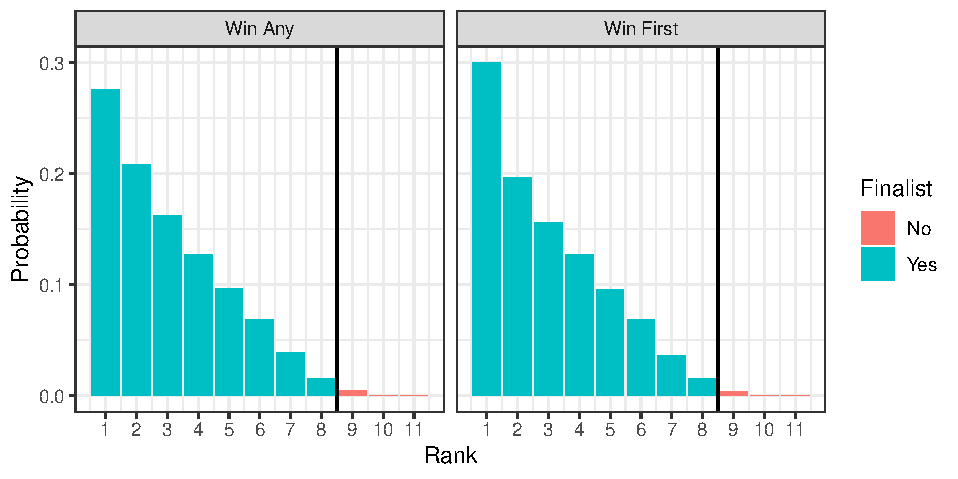
\includegraphics{draft_files/figure-latex/unnamed-chunk-7-1.pdf}
\caption{Boxplots of scoring distribution for every qualification rank}
\end{figure}

\hypertarget{drawbacks-of-the-scoring-system}{%
\subsection{Drawbacks of the scoring
system}\label{drawbacks-of-the-scoring-system}}

\hypertarget{sum-of-ranks-instead-of-product}{%
\subsubsection{Sum of ranks instead of
product}\label{sum-of-ranks-instead-of-product}}

We performed the same tasks as we did for products

Probabilities of advancing, winning medals are all lower

Most notably for qualifications,

Obvious that the average score between the ranks are closer to each
other

The amount of variability doesn't seem to be different as the rank
increases

\hypertarget{speed-climbing-vs-lead-and-bouldering}{%
\subsubsection{Speed climbing vs lead and
bouldering}\label{speed-climbing-vs-lead-and-bouldering}}

For our analysis on the relationship between the rankings of the events
and the final result, we used data from the 2018 Youth Olympics Women's
Qualification. Figure 3 is a scatterplot and correlation matrix between
the ranks of the individual events and the final standings, with
Kendall's Tau (Kendall Rank Correlation Coefficient) as our measure of
ordinal association between the quantities. It is evidently clear that
there is a strong and positive correlation between the ranks of
bouldering and lead climbing, and as a results, the standings of these
two events are highly correlated with the final rankings. On the other
hand, the correlation with the final rank is not as strong for speed
climbing. Thus, speed climbers are facing a huge disadvantage in this
scoring system, compared to those that are specialized in the other two
concentrations.

This trend also holds for most of the past competitions.

\begin{figure}
\centering
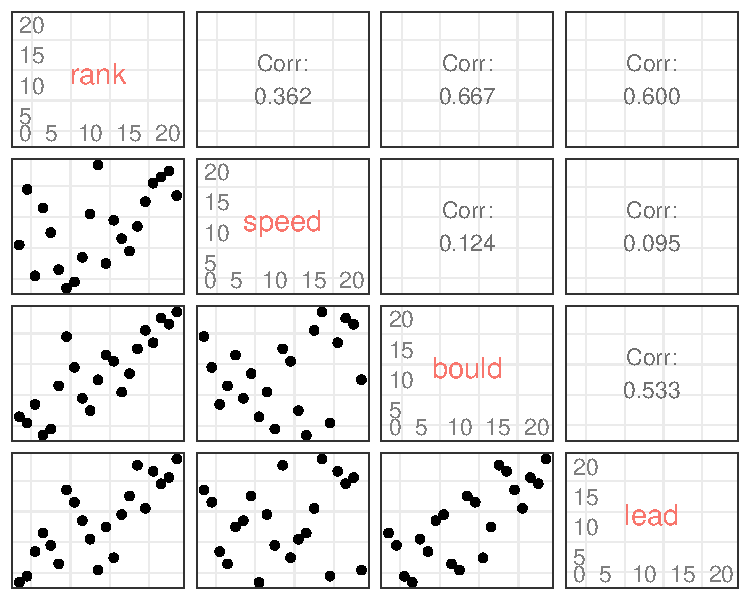
\includegraphics{draft_files/figure-latex/unnamed-chunk-9-1.pdf}
\caption{Kendall's rank correlations - 2018 World Championship, Women's
Qualification}
\end{figure}

\hypertarget{drop-and-re-rank}{%
\subsubsection{Drop and re-rank}\label{drop-and-re-rank}}

A single climber excluded changes things drastically, especially order
of medalists.

The cases where someone behind you drops out and your ranking changes.

Example from 2018 youth, women's final dropping ranks 3 and 5 change the
medalist order

\begin{figure}
\centering
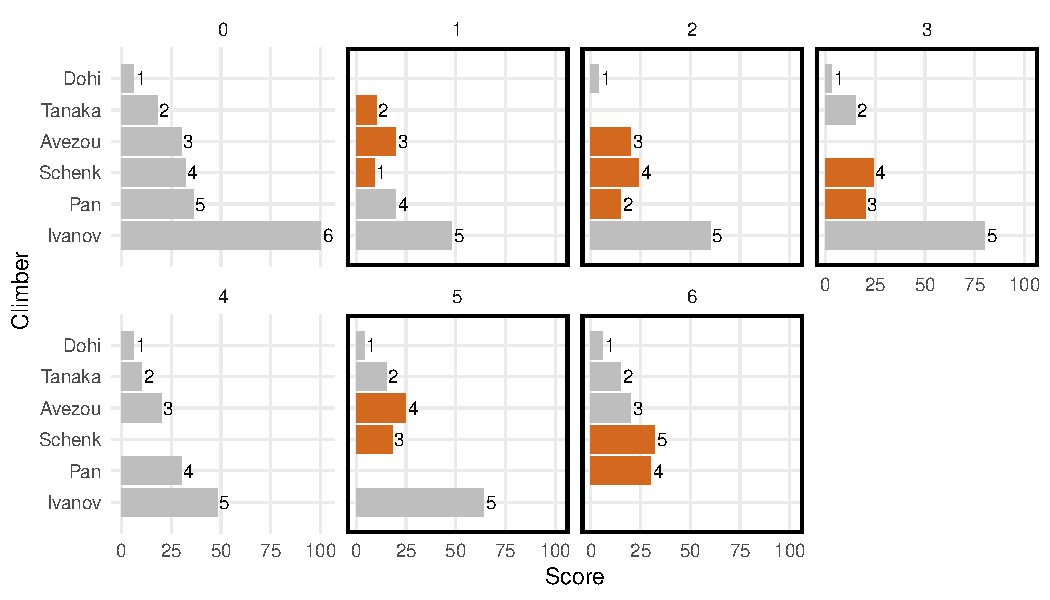
\includegraphics{draft_files/figure-latex/unnamed-chunk-11-1.pdf}
\caption{Original rankings and rankings after each rank is dropped}
\end{figure}

\bibliographystyle{agsm}
\bibliography{}

\end{document}
